%{{{Header
\documentclass[a4paper,11pt]{article}
\usepackage{anysize}
\marginsize{2cm}{2cm}{1cm}{1cm}
%\textwidth 6.0in \textheight = 664pt
\usepackage{xltxtra}
\usepackage{mathtools}
\usepackage{amsmath}
\usepackage{graphicx}
\usepackage{color}
\usepackage{xgreek}
\usepackage{fancyvrb}
\usepackage{minted}
\usepackage{listings}
\usepackage{hyperref}
\usepackage[noend]{algpseudocode}
\usepackage{algorithm}
\usepackage{enumitem}
\usepackage{framed}
\usepackage{relsize}
\usepackage{float}
\setmainfont[Mapping=TeX-text]{DejaVu Serif}
\newcommand{\tab}{\hspace*{3em}}

%\setsansfont{FreeSans}
%\setmonofont{FreeMono}
\begin{document}
%\def\thesubsection {\alph{subsection}}
\renewcommand{\labelenumi}{\roman{enumi})}
\renewcommand{\labelenumii}{\arabic{enumii}.}

\begin{titlepage}
\begin{center}


\includegraphics[width=0.15\textwidth]{title/Pyrforos2.png}\\[1.cm]
\textsc{\LARGE Εθνικό Μετσόβιο Πολυτεχνείο}\\[1.5cm]

\Large{ Αναφορά Εξαμηνιαίου Project }\\[0.5cm]

% Title
\begin{doublespace}
\HRule \\[0.4cm]
{\huge \bfseries
Βάσεις Δεδομένων
}\\[0.4cm]
Σχεδιασμοί Βάσεων Δεδομένων\\
\end{doublespace}

\HRule \\[1.5cm]

\begin{minipage}{0.4\textwidth}
\begin{flushleft} \large
\begin{tabular}{l l}
Βασίλης \textsc{Γερακάρης} & (08092)\\
Διονύσης \textsc{Ζήνδρος} & (06601)\\
Γρηγόρης \textsc{Λύρας}	& (09687)\\
\end{tabular}
\end{flushleft}
\end{minipage}
\begin{minipage}{0.4\textwidth}
\begin{flushright} \large
\emph{Διδάσκοντες:} \\
Γιάννης \textsc{Βασιλείου}\\
Τίμος \textsc{Σελλής}
\end{flushright}
\end{minipage}

\vfill

{\large \today}
\end{center}
\end{titlepage}

%}}}

%{{{ Άσκηση 1
\section{Άσκηση 1} \setcounter{section}{1}

Μας δίνεται το παρακάτω $B^+$ δέντρο και καλούμαστε να το σχεδιάσουμε μετά τη
διαγραφή της τιμής $43^*$:
\begin{figure}[h]
\centering
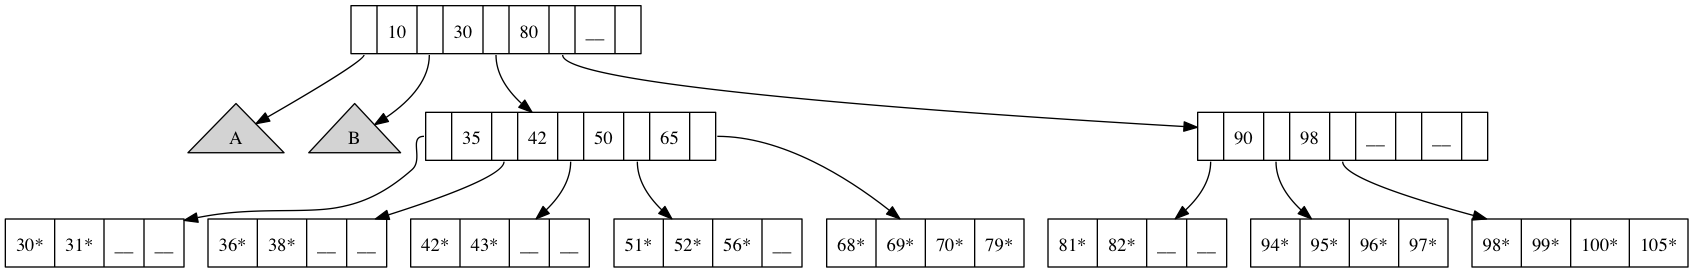
\includegraphics[width=1\textwidth]{../files/init_tree.png}\\
\caption{Αρχικό δέντρο.}
\end{figure}

\subsection {Συγχώνευση με δεξιό αδελφό}
Στην περίπτωση συγχώνευσης με το δεξιό αδελφό, το $42^*$ καταλαμβάνει την
πρώτη θέση του νέου φύλλου. Αφού έγινε συγχώνευση θα πρέπει να διαγραφεί η
καταχώρηση που έδειχνε στο sibling (50) από τον κόμβο-πατέρα. Το δέντρο που
προκύπτει είναι το παρακάτω:

\begin{figure}[h]
\centering
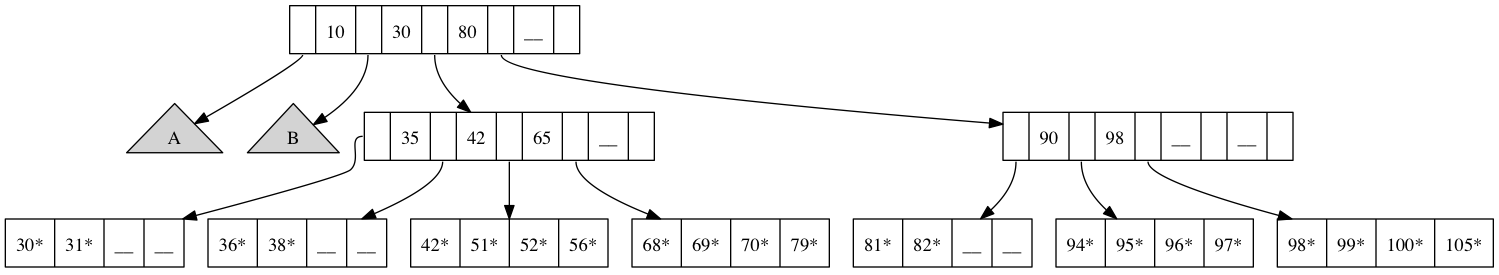
\includegraphics[width=1\textwidth]{../files/tree1a.png}\\
\caption{Μετά από συγχώνευση δεξιά.}
\end{figure}

\subsection {Συγχώνευση με αριστερό αδελφό}
Στην περίπτωση συγχώνευσης αριστερά, το $42^*$ θα καταλάβει την
3\textsuperscript{η} θέση του φύλλου. Αφού έγινε συγχώνευση, θα πρέπει να
διαγραφεί η καταχώρηση που έδειχνε στο 42 από τον κόμβο-πατέρα. Το δέντρο που
προκύπτει φαίνεται παρακάτω:

\begin{figure}[h]
\centering
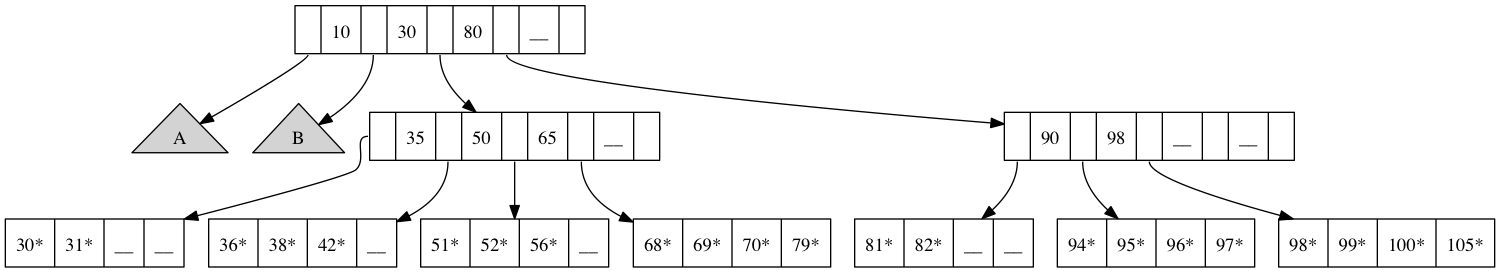
\includegraphics[width=1\textwidth]{../files/tree1b.png}\\
\caption{Μετά από συγχώνευση αριστερά.}
\end{figure}

\pagebreak

\subsection {Ανακατανομή εγγραφών με δεξιό αδελφό}
Στην περίπτωση ανακατανομής εγγραφών με το δεξιό αδελφό, το $51^*$ μεταφέρεται
και καταλαμβάνει τη θέση που έμεινε κενή από τη διαγραφή. Αφού έγινε
ανακατανομή, η μεσαία εγγραφή του φύλλου που περιείχε το sibling που θα
μεταφερθεί (52) ανεβαίνει ως κλειδί στον κόμβο-πατέρα. Το δέντρο που προκύπτει
είναι το παρακάτω:

\begin{figure}[h]
\centering
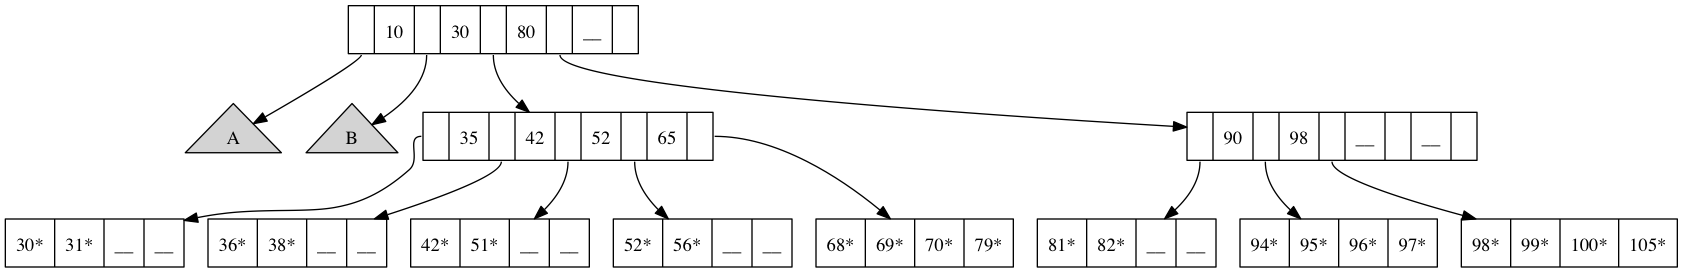
\includegraphics[width=1\textwidth]{../files/tree1c.png}\\
\caption{Μετά από ανακατανομή εγγραφών.}
\end{figure}

Και στις 3 περιπτώσεις, η διαγραφή του $43^*$ καθιστά τον κομβο-φύλλο λιγότερο
από μισο-γεμάτο, επομένως απαιτεί συγχώνευση ή ανακατανομή, που αυξάνουν το
κόστος.
Στο παράδειγμά μας παρατηρούμε ότι ο δεξιός αδερφός δεν είναι
minimal-sized, επομένως (στη γενική περίπτωση) μας συμφέρει από άποψη κόστους
να πραγματοποιήσουμε ανακατανομή των φύλλων με αυτόν. Με τον τρόπο αυτό δε
χρειάζεται να διαγράψουμε τιμές από τον κόμβο-πατέρα (απλώς αλλαγή ενός
κλειδιού). Επιπλέον, το αποτέλεσμα είναι ευνοϊκό για μελλοντικές εισαγωγές
δεδομένων, αφού έχουμε ώς αποτέλεσμα 3 minimal-sized κόμβους-φύλλα, επομένως
δε θα χρειαστεί να πραγματοποιηθεί διάσπαση κατά την εισαγωγή.

Στην περίπτωση που είχαμε να πραγματοποιήσουμε σχεδόν αποκλειστικά διαγραφές
εγγραφών, η συγχώνευση με ένα sibling θα ήταν προτιμότερη, αφού θα μείωνε τον
αριθμό των κλειδιών του κόμβου-πατέρα και θα οδηγούμασταν γρηγορότερα σε
μείωση του ύψους του δέντρου.

%}}}

%{{{ Άσκηση 2
\section{Άσκηση 2}
Το δέντρο της παραπάνω άσκησης ευρετηριοποιεί μια σχέση R, επομένως τα φύλλα
περιέχουν δείκτες προς το αρχείο. Το δέντρο πρέπει να είναι ισσοροπημένο,
οπότε προκύπτει ότι τα Α,Β είναι κόμβοι και όχι φύλλα. Καθώς είναι όσο το
δυνατόν πιο άδεια, θεωρούμε ότι το κάθε ένα έχει 2 μόνο τιμές (50\% πληρότητα)
άρα 3 δείκτες σε φύλλα. Κάθε φύλλο περιέχει 2 μόνο κλειδιά.

Σε επίπεδο φύλλων έχουμε λοιπόν $6 + 6 + 23 = 35$ δείκτες σε blocks του δίσκου.
Κάθε block χωράει 20 εγγραφές της R, επομένως συνολικά υπάρχουν
$20 \times 35 = 700$ πλειάδες.
\pagebreak
%}}}

%{{{ Άσκηση 3
\section{Άσκηση 3}

Το γνώρισμα Α, ως κλειδί, παίρνει \emph{όλες} τις τιμές από 0 - 5.999.999,
αφού υπάρχουν 6.000.000 εγγραφές.

\begin{enumerate}
    \item \underline{Απ'ευθείας προσπέλαση στο δίσκο}
    \begin{enumerate}
	\item Θα διαβαστούν σειριακά όλες οι εγγραφές ως την Α = 59.999, οπότε
	θα χρειαστούν συνολικά $60.000/10 = \textbf{6.000}$ I/Os
	\item Αφού τα δεδομένα είναι σειριακά ταξινομημένα στο δίσκο μπορούμε
	να εφαρμόσουμε δυαδική αναζήτηση στα blocks του δίσκου. Οι αναζητήσεις
	μας θα είναι στη μορφή:\\ 3.000.000 -> 1.500.000 -> 750.000 -> 375.000
	-> 187.500 -> 93.750 -> 46.875 -> 70.313 -> 58594 -> 52.734 -> ...\\
	Επομένως $\log_2600.000 = \textbf{20}$ I/Os
	\item Δυαδική αναζήτηση ώς το 60.000 και μετά σειριακή ανάγνωση blocks.
	θα χρειαστούν συνολικά $\log_2600.000 + 1= \textbf{21}$ I/Os
	\item Θα προσπελαστεί όλο το αρχείο, επομένως απαιτούνται $6.000.000/10
	= \textbf{600.000}$ I/Os
    \end{enumerate}

    \item \underline{Χρήση $B^+$ δέντρου}\\
    Θεωρούμε σε κάθε περίπτωση ότι το δέντρο είναι γεμάτο. Κάθε φύλλο έχει τη
    δυνατότητα να αποθηκεύσει ως 100 δείκτες σε εγγραφές. Απαιτούνται για την
    αναπαράσταση των εγγραφών συνολικά: $6.000.000/100 = 60.000$ φύλλα.\\
    Το από πάνω επίπεδο (αφού κάθε κόμβος έχει 100 δείκτες) θα έχει:\\
    $60.000/100 = 600$ κόμβους.\\
    Στο ακόμη παραπάνω επίπεδο χρειάζονται: $600/100 = 6$ κόμβοι.\\
    Τέλος, αρκεί ένας κόμβος-ρίζα για να δείχνει στους 6 αυτούς κόμβους.\\
    Το δέντρο λοιπόν σχηματίζεται από 4 επίπεδα και απαιτούνται συνολικά:\\
    $60.000 + 600 + 6 + 1 = 60.607$ blocks.

    \begin{enumerate}
	\item To $1^o$ φύλλο περιέχει τις εγγραφές 0-99, το $2^o$ τις 100-199
	κλπ. Η τιμή Α = 60.000 είναι στο $600^o$ φύλλο. Θα χρειαστεί να γίνει
	ανάγνωση από τη ρίζα, από το παιδί της στο $2^o$ επίπεδο, από το παιδί
	στο $3^o$ επίπεδο και έπειτα τα 599 πρώτα φύλλα.\\
	Συνολικά: $1 + 1 + 1 + 599 = \textbf{602}$ I/Os
	\item Θα πρέπει να διαβαστούν η ρίζα, το κατάλληλο παιδί στο $2^o$
	επίπεδο, το κατάλληλο στο $3^o$ επίπεδο και τέλος το φύλλο που
	περιέχει την εγγραφή Α=60.000\\
	Θα χρειαστούν λοιπόν \textbf{4} I/Os \emph{(height+1)}.
	\item Όπως δείξαμε πριν, το $600^o$ φύλλο περιέχει τις εγγραφές
	60.000-60099. Άρα, θα διαβαστεί η ρίζα, το κατάλληλο παιδί στο $2^o$
	επίπεδο, το κατάλληλο στο $3^o$ επίπεδο και το $600^o$ φύλλο.\\
	Απαιτούνται επομένως \textbf{4} I/Os.
	\item Θα χρειαστεί να προσπελάσουμε όλα τα φύλλα του δέντρου για να
	υπολογίσουμε το αποτέλεσμα, μαζί με τα I/Os για τη ρίζα και τo πρώτo
	παιδί για τα επόμενα 2 επίπεδα.\\
	Συνολικά χρειάζονται: $1 + 1 + 1 + 60.000 = \textbf{60.003}$ I/Os.
    \end{enumerate}
    \pagebreak

    \item \underline{Χρήση μη-δυναμικού κατακερματισμού}\\
    Αφού ο κατακερματισμός γίνεται ως υπερχείληση, θα χρησιμοποιηθούν συνολικά
    $6.000.000 / 10 = 600.000$ buckets που θα είναι τελείως πλήρη. Ως hash
    function για την κατανομή αυτή επιλέγεται η $h(A) = A \mod 600.000$.
    \begin{enumerate}
	\item Οι ζητούμενες εγγραφές βρίσκονται στα πρώτα 60.000 (0 - 59.999)
	buckets, επομένως απαιτούνται \textbf{60.000} I/Os.
	\item Η πλειάδα αυτή βρίσκεται περνώντας την τιμη στη hash function
	h(A), που μας οδηγεί απευθείας στο $60.001^o$ bucket.\\
	Χρειάζεται \emph{μόνο} \textbf{1} I/O (φαίνεται η ισχύς του
	κατακερματισμού σε equality queries)
	\item Οι ζητούμενες εγγραφές βρίσκονται στους κάδους 60.001-60.009,
	επομένως θα χρειαστούν \textbf{9} λειτουργίες I/O
	\item Θα χρειαστεί να προσπελάσουμε όλα τα buckets για να υπολογιστεί
	το αποτέλεσμα, επομένως και όλα τα blocks.\\
	Συνολικά χρειάζονται: \textbf{600.000} I/Os
    \end{enumerate}
\end{enumerate}

%}}}

%{{{ Άσκηση 4
\section{Άσκηση 4}

\subsection*{(α)}
Ο μέγιστος αριθμός block δίσκου που μπορεί να χρησιμοποιηθούν για την
αποθήκευση των 100.000 εγγραφών είναι 1990.

Στη χειρότερη περίπτωση, θα υπάρχει 1 μόνο record σε κάθε bucket εκτός από
ένα. Στο τελευταίο αυτό bucket θα πρέπει να αποθηκευτούν $100.000 - 999 =
99.001$ εγγραφές. Αφού κάθε block χωράει ως 100 εγγραφές, θα χρειαστούν 991
blocks για το συγκεκριμένο bucket (1 κανονικό + 990 overflow). Συνολικά 1990.

Το αποτέλεσμα αυτό προκύπτει πιθανώς και με άλλο τρόπο. Γεμίζοντας 990 buckets
με 100 records έκαστο και έπειτα βάζοντας ένα overflow bucket με ένα στοιχείο
στο καθένα. Έτσι, έχουν αποθηκευτεί 99990 εγγραφές. Σε κάθε ένα από τα
υπολοιπόμενα buckets τοποθετούμε από μια εγγραφή. Με τον τρόπο αυτό, έχουμε
χρησιμοποιήσει $2\times 990 + 10 = 1990$ blocks δίσκου.

\subsection*{(β)}
Ο ελάχιστος αριθμός block δίσκου που μπορούν να χρησιμοποιηθούν είναι 1000.
Αυτό συμβαίνει στην απολύτως ιδανική περίπτωση όπου οι εγγραφές χωρίζονται
ακριβώς, από 100 σε κάθε bucket. Τότε, χρειαζόμαστε μόνο 1 block για το
καθένα, δηλαδή συνολικά 1000.

\subsection*{(γ)}
Στην περίπτωση των 100.099 εγγραφών, θα εργαστούμε με παρόμοιο τρόπο με το
(α). Γεμίζοντας 991 buckets με 100 στοιχεία και τοποθετώντας ένα overflow
bucket με ένα στοιχείο στο καθένα, έχουμε συνολικά αποθηκεύσει 100.091
εγγραφές. Τις υπόλοιπες 8 εγγραφές τις αποθηκεύουμε από μία σε 8 από τα 9
υπολοιπόμενα buckets. Για το σενάριο αυτό, συνολικά απαιτούνται $2\times 991 +
8 = 1990$ blocks δίσκου, η ίδια απάντηση με το (α). (Το ίδιο αποτέλεσμα
προκύπτει αν γεμίσουμε 999 buckets με ένα record και τοποθετήσουμε όλα τα
υπολοιπα στο τελευταίο bucket.
%}}}

\end{document}
